% ============================================================
%  Rapport de Stage de Fin d'Etudes
%  Rayen -- Tunisie Telecom
%  Annee universitaire 2025/2026
% ============================================================
\documentclass[12pt,a4paper]{report}

\usepackage[french]{babel}
\usepackage[utf8]{inputenc}
\usepackage[T1]{fontenc}
\usepackage[a4paper,left=2.5cm,right=2.5cm,top=3cm,bottom=2.5cm,headheight=60pt]{geometry}
\usepackage{graphicx}
\usepackage{fancyhdr}
\usepackage{titlesec}
\usepackage[hidelinks,colorlinks=true,linkcolor=blue,citecolor=blue,urlcolor=blue]{hyperref}
\usepackage{xcolor}
\usepackage{enumitem}
\usepackage{caption}
\usepackage{subcaption}
\usepackage{float}
\usepackage{setspace}
\usepackage{tikz}
\usetikzlibrary{shapes.geometric,arrows.meta,positioning,fit,backgrounds}
\usepackage{tabularx}
\usepackage{booktabs}
\usepackage{listings}
\usepackage{lastpage}
\usepackage{amsmath}
\usepackage{microtype}

\definecolor{ttblue}{RGB}{31,73,125}
\definecolor{codegreen}{rgb}{0.0,0.5,0.0}
\definecolor{codegray}{rgb}{0.5,0.5,0.5}
\definecolor{backcolor}{rgb}{0.97,0.97,0.97}

\titleformat{\chapter}[display]
  {\normalfont\bfseries\Large\color{ttblue}}
  {\Large\chaptertitlename\ \thechapter\ :}{6pt}{\Large}
\titlespacing*{\chapter}{0pt}{0pt}{30pt}
\titleformat{\section}
  {\normalfont\bfseries\large\color{ttblue}}{\thesection.}{0.6em}{}
\titleformat{\subsection}
  {\normalfont\bfseries\normalsize}{\thesubsection.}{0.6em}{}
\titleformat{\subsubsection}
  {\normalfont\bfseries\small}{\thesubsubsection.}{0.6em}{}

\pagestyle{fancy}
\fancyhf{}
\renewcommand{\headrulewidth}{0.6pt}
\fancyhead[L]{\small\textit{Rapport de Stage --- Tunisie Telecom}}
\fancyhead[R]{\small\textit{2025/2026}}
\fancyfoot[C]{\thepage\ / \pageref{LastPage}}
\fancypagestyle{plain}{
  \fancyhf{}
  \fancyhead[L]{\small\textit{Rapport de Stage --- Tunisie Telecom}}
  \fancyhead[R]{\small\textit{2025/2026}}
  \fancyfoot[C]{\thepage\ / \pageref{LastPage}}
  \renewcommand{\headrulewidth}{0.6pt}
}

\lstset{
  backgroundcolor=\color{backcolor},
  basicstyle=\ttfamily\small,
  keywordstyle=\color{ttblue}\bfseries,
  commentstyle=\color{codegreen}\itshape,
  frame=single,breaklines=true,columns=fullflexible,
  showstringspaces=false,
  numbers=left,numberstyle=\tiny\color{codegray},numbersep=5pt
}

\tikzstyle{block}=[rectangle,rounded corners=3pt,minimum width=3.2cm,
  minimum height=0.85cm,text centered,draw=ttblue,fill=blue!5,
  font=\small,text width=3cm]
\tikzstyle{blockW}=[rectangle,rounded corners=3pt,minimum width=4.2cm,
  minimum height=0.85cm,text centered,draw=ttblue,fill=blue!5,
  font=\small,text width=4cm]
\tikzstyle{store}=[cylinder,shape border rotate=90,draw=gray!60,fill=gray!10,
  font=\small,minimum height=1.1cm,minimum width=2.8cm,text centered,text width=2.6cm]
\tikzstyle{arrow}=[-{Stealth[length=5pt]},thick,color=ttblue!80]
\tikzstyle{dasharrow}=[-{Stealth[length=5pt]},dashed,thick,color=gray!55]

\begin{document}

% ============================================================
% PAGE DE GARDE
% ============================================================
\begin{titlepage}
\thispagestyle{empty}
\begin{center}
\vspace*{1.5cm}
{\large\bfseries\color{ttblue} RAPPORT DE STAGE DE FIN D'\'ETUDES}\\[0.5cm]
\rule{\textwidth}{1.5pt}\\[0.4cm]
{\LARGE\bfseries Analyse automatique des journaux Oracle\\[0.3cm]
par G\'en\'eration Augment\'ee par R\'ecup\'eration (RAG)}\\[0.4cm]
\rule{\textwidth}{1.5pt}
\vspace{2.2cm}
\begin{tabular}{ll}
\textbf{\'Elabor\'e par :}        & Rayen \\[0.3cm]
\textbf{Encadr\'e par :}          & Monsieur Ben Mohamed Ahmed \\[0.15cm]
                                   & \small Chef de la Subdivision Administration \\[0.15cm]
                                   & \small Syst\`emes et Bases de Donn\'ees \\[0.3cm]
\textbf{Soci\'et\'e d'accueil :}  & Tunisie Telecom -- Centre technique IT de la Kasbah \\[0.3cm]
\textbf{D\'epartement :}          & Direction Centrale des Syst\`emes d'Information (DCSI) \\[0.3cm]
\textbf{Ann\'ee universitaire :}  & 2025/2026 \\
\end{tabular}
\vfill
{\color{ttblue}\rule{0.4\textwidth}{0.8pt}}
\end{center}
\end{titlepage}

% ============================================================
% REMERCIEMENTS
% ============================================================
\chapter*{Remerciements}
\addcontentsline{toc}{chapter}{Remerciements}

Je tiens tout d'abord \`a adresser mes sinc\`eres remerciements \`a l'ensemble du personnel
de Tunisie Telecom, et plus particuli\`erement \`a celui du centre technique IT de la Kasbah,
pour l'accueil chaleureux qui m'a \'et\'e r\'eserv\'e durant toute la dur\'ee de mon stage.

Mes remerciements les plus sinc\`eres vont \`a mon encadreur, Monsieur Ben Mohamed
Ahmed, Chef de la Subdivision Administration Syst\`emes et Bases de Donn\'ees, qui
m'a accord\'e sa confiance d\`es le premier jour. Sa disponibilit\'e constante, la pertinence
de ses conseils et son expertise technique m'ont \'enorm\'ement apport\'e et ont grandement
contribu\'e \`a la r\'eussite de ce stage.

Je souhaite \'egalement exprimer ma gratitude \`a Monsieur Mustapha Charfeddine
Akkez, dont les conseils avis\'es et le soutien de tous les instants m'ont accompagn\'e tout
au long de cette exp\'erience.

Plus g\'en\'eralement, je remercie chaleureusement toutes les personnes qui, de pr\`es ou
de loin, m'ont fait profiter de leur savoir-faire et de leur exp\'erience durant ce stage.

% ============================================================
% TABLE DES MATIERES
% ============================================================
\tableofcontents
\listoffigures
\listoftables

% ============================================================
% INTRODUCTION GENERALE
% ============================================================
\chapter*{Introduction g\'en\'erale}
\addcontentsline{toc}{chapter}{Introduction g\'en\'erale}

Dans le cadre de ma formation d'ing\'enieur, j'ai effectu\'e un stage au sein du centre
technique IT de la Kasbah de Tunisie Telecom, rattach\'e \`a la Direction Centrale des
Syst\`emes d'Information (DCSI). Ce stage s'est d\'eroul\'e au cours du premier semestre
de l'ann\'ee universitaire 2025/2026 et m'a permis d'aborder des probl\'ematiques
concr\`etes li\'ees \`a l'administration des bases de donn\'ees Oracle, un environnement
que Tunisie Telecom exploite \`a grande \'echelle pour assurer la continuit\'e de ses services.

L'un des d\'efis quotidiens des \'equipes DBA (\textit{Database Administrators}) est
l'analyse des journaux d'erreurs produits par Oracle Database. Ces fichiers,
appel\'es \emph{alert logs}, accumulent des milliers de lignes par jour et signalent des
\'ev\'enements aussi vari\'es qu'une saturation d'espace disque, un verrou
(\emph{deadlock}), une interruption du processus d'archivage ou encore une erreur de
connexion. Face au volume de ces journaux, le temps consacr\'e \`a leur lecture manuelle
repr\'esente une charge non n\'egligeable pour les \'equipes techniques.

L'objectif de ce stage \'etait donc de concevoir et de d\'evelopper un syst\`eme capable
d'analyser automatiquement ces fichiers, d'identifier les codes d'erreur pr\'esents, d'en
expliquer la signification et de proposer des actions correctives. Pour cela, j'ai retenu
l'approche dite de \emph{G\'en\'eration Augment\'ee par R\'ecup\'eration}
(RAG, \textit{Retrieval-Augmented Generation}), qui combine une base de connaissances
structur\'ee avec un mod\`ele de g\'en\'eration de texte, afin d'ancrer les explications
produites sur des faits v\'erifiables plut\^ot que sur de simples suppositions.

Ce rapport est organis\'e en trois chapitres. Le premier pr\'esente l'entreprise d'accueil,
Tunisie Telecom, ainsi que le d\'epartement DCSI au sein duquel j'ai travaill\'e. Le
deuxi\`eme chapitre d\'ecrit l'architecture d'Oracle Database en s'attardant plus
particuli\`erement sur la structure de ses journaux d'erreurs, point de d\'epart de tout le
traitement mis en place. Enfin, le troisi\`eme chapitre d\'etaille le syst\`eme RAG con\c cu et
impl\'ement\'e~: construction de la base de connaissances, algorithmes de r\'ecup\'eration,
g\'en\'eration des explications et exp\'erimentations men\'ees. Le rapport se conclut par un
bilan des apports du stage et des perspectives d'am\'elioration envisag\'ees.

% ============================================================
% CHAPITRE 1 : PRESENTATION DE TUNISIE TELECOM
% ============================================================
\chapter{Pr\'esentation de Tunisie Telecom et du d\'epartement DCSI}

\section{Aper\c cu historique}

L'Office national des t\'el\'ecommunications, plus connu par sa d\'enomination commerciale
Tunisie Telecom, a \'et\'e cr\'e\'e par la loi n\textdegree{}36 du 17 avril 1995~; loi qui
entrera en vigueur le 1\textsuperscript{er} janvier 1996. Quelques ann\'ees plus tard, fin
2002, Tunisie Telecom devient une soci\'et\'e anonyme de droit public.

Depuis sa cr\'eation, Tunisie Telecom \oe{}uvre \`a consolider l'infrastructure des
t\'el\'ecoms en Tunisie et \`a am\'eliorer le taux de p\'en\'etration. Elle a inaugur\'e sa
premi\`ere ligne GSM le 20 mars 1998. \`A partir de cette date, l'entreprise conna\^itra
d'importantes \'evolutions dans tous les domaines, notamment technologique, commercial et
marketing.

En mai 2000, Tunisie Telecom met en place, exploite et commercialise le premier r\'eseau
GSM hors des fronti\`eres nationales, plus pr\'ecis\'ement en Mauritanie (MATTEL). Elle
lance ensuite, en 2009, le 1\textsuperscript{er} c\^able sous-marin 100\,\% tunisien
d\'enomm\'e Hannibal. La m\^eme ann\'ee conna\^it un autre \'ev\'enement majeur~: le
lancement d'Elissa, marque con\c cue exclusivement pour les jeunes de moins de 25 ans,
qui sera \'etendue en 2012 \`a tous sans limite d'\^age.

En 2011, Tunisie Telecom lance son r\'eseau 3G~; cinq ans plus tard, en 2016, ce sera au
tour de la 4G. Aujourd'hui, l'op\'erateur se compose de 24 directions r\'egionales, de
140~Espaces TT et de plus de 13\,000 points de vente priv\'es. Il dispose de
3~data centers r\'epondant aux normes internationales, emploie pr\`es de 6\,400 agents
et h\'eberge 7~filiales dont Sotetel, Topnet et l'ATI (Agence Tunisienne de l'Internet).

\section{Domaine d'activit\'es}

Tunisie Telecom propose des services dans le domaine des t\'el\'ecommunications fixes et
mobiles, parmi lesquels~:

\begin{itemize}[leftmargin=*]
  \item L'installation, le d\'eveloppement, l'entretien et l'exploitation des r\'eseaux
        publics de t\'el\'ecommunications~;
  \item La promotion et la commercialisation de services \`a valeur ajout\'ee~: internet
        haut d\'ebit, IPTV, solutions cloud pour entreprises~;
  \item La fourniture de solutions d'interconnexion et de transit international \`a
        travers ses c\^ables sous-marins~;
  \item L'h\'ebergement et la gestion d'infrastructures informatiques critiques au sein
        de ses data centers certifi\'es Tier~III.
\end{itemize}

\section{Organigramme g\'en\'eral}

La figure~\ref{fig:organigramme} pr\'esente la structure organisationnelle de haut niveau
de Tunisie Telecom. On y distingue deux grands axes~: d'une part les directions
fonctionnelles rattach\'ees directement au Pr\'esident-Directeur G\'en\'eral (PDG), et
d'autre part les directions op\'erationnelles et commerciales plac\'ees sous l'autorit\'e
du Directeur G\'en\'eral Adjoint (DGA). Parmi les directions centrales repr\'esent\'ees,
c'est la \textbf{Direction Centrale des Syst\`emes d'Information (DCSI)} qui constitue
le cadre principal de ce stage.

\begin{figure}[H]
  \centering
  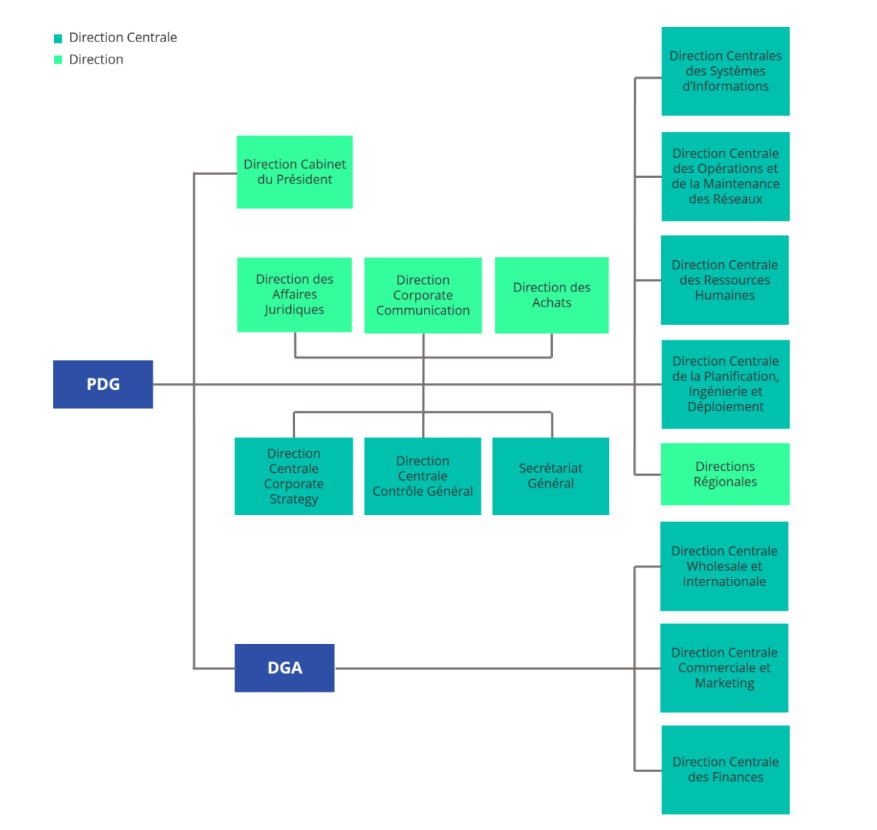
\includegraphics[width=0.95\textwidth]{images/organigramme_tt.png}
  \caption{Organigramme g\'en\'eral de Tunisie Telecom}
  \label{fig:organigramme}
\end{figure}

\section{La Direction Centrale des Syst\`emes d'Information (DCSI)}

La DCSI est responsable de la mise en \oe{}uvre et de la maintenance de l'ensemble
de l'infrastructure informatique de Tunisie Telecom. Son p\'erim\`etre couvre les
r\'eseaux internes, la s\'ecurit\'e des syst\`emes ainsi que l'administration des
serveurs et des bases de donn\'ees. Elle est organis\'ee autour de plusieurs services
compl\'ementaires.

\subsection{Service r\'eseau informatique}

Ce service prend en charge l'ensemble des r\'eseaux internes de l'entreprise~: r\'eseaux
locaux (LAN), r\'eseaux \'etendus (WAN), t\'el\'ephonie d'entreprise, intranet et acc\`es
internet. Il d\'efinit les proc\'edures d'interconnexion des \'equipements (routeurs,
commutateurs) et veille \`a leurs performances au quotidien.

\subsection{Service s\'ecurit\'e informatique}

Ce service assure la protection des donn\'ees et des syst\`emes de l'entreprise autour
de trois axes principaux~:

\begin{itemize}[leftmargin=*]
  \item \textbf{Confidentialit\'e}~: seules les personnes habilit\'ees acc\`edent aux
        informations qui leur sont destin\'ees~;
  \item \textbf{Authentification}~: chaque utilisateur s'identifie avant d'acc\'eder
        aux ressources du syst\`eme d'information~;
  \item \textbf{Disponibilit\'e et int\'egrit\'e}~: les donn\'ees h\'eberg\'ees dans
        les data centers sont prot\'eg\'ees contre toute alt\'eration ou perte accidentelle.
\end{itemize}

\subsection{Service administration syst\`eme et bases de donn\'ees}

C'est au sein de ce service que j'ai effectu\'e mon stage. Ses missions principales sont~:

\begin{itemize}[leftmargin=*]
  \item La supervision proactive des instances Oracle en production~;
  \item L'analyse des journaux d'erreurs pour d\'etecter et traiter les incidents~;
  \item La gestion des sauvegardes et des restaurations via RMAN~;
  \item L'application des correctifs de s\'ecurit\'e et des mises \`a jour de versions.
\end{itemize}

C'est pr\'ecis\'ement la charge li\'ee \`a l'analyse manuelle des journaux d'erreurs qui
a motiv\'e le sujet de ce stage.

% ============================================================
% CHAPITRE 2 : ORACLE DATABASE ET SES JOURNAUX
% ============================================================
\chapter{Architecture d'Oracle Database et structure des journaux}

\section{Vue d'ensemble d'Oracle Database}

Oracle Database est l'un des syst\`emes de gestion de bases de donn\'ees relationnelles
(SGBDR) les plus utilis\'es dans les environnements d'entreprise \`a travers le monde.
Son architecture repose sur une s\'eparation nette entre deux entit\'es~: l'instance
Oracle d'un c\^ot\'e, et la base de donn\'ees physique de l'autre. Cette distinction
est fondamentale pour comprendre comment Oracle g\`ere et journalise ses erreurs.

\subsection{La base de donn\'ees physique}

Sur disque, une base de donn\'ees Oracle se compose des cat\'egories de fichiers suivantes~:

\begin{itemize}[leftmargin=*]
  \item \textbf{Fichiers de donn\'ees} (\emph{datafiles})~: stockent les donn\'ees
        applicatives~--- tables, index, vues mat\'erialis\'ees, proc\'edures stock\'ees~;
  \item \textbf{Fichiers de journalisation} (\emph{redo log files})~: enregistrent en
        continu toutes les modifications apport\'ees \`a la base, valid\'ees ou non. Le
        processus LGWR (\emph{Log Writer}) est responsable de leur alimentation~;
  \item \textbf{Fichiers de contr\^ole} (\emph{control files})~: contiennent les
        m\'etadonn\'ees critiques de la base~: nom, emplacement des fichiers, SCN
        (\emph{System Change Number}) courant~;
  \item \textbf{Fichier de param\`etres} (\emph{spfile}/\emph{pfile})~: d\'efinit les
        param\`etres de l'instance au d\'emarrage~;
  \item \textbf{Fichiers d'archivage} (\emph{archived redo logs})~: copies des redo log
        files apr\`es remplissage, conserv\'ees pour une r\'ecup\'eration compl\`ete.
\end{itemize}

\subsection{L'instance Oracle}

L'instance Oracle est l'ensemble des processus et structures m\'emoire qui permettent
l'acc\`es \`a la base de donn\'ees.

\subsubsection{Les zones m\'emoire}

\begin{itemize}[leftmargin=*]
  \item \textbf{SGA (System Global Area)}~: zone m\'emoire partag\'ee par tous les
        utilisateurs connect\'es. Elle contient le \emph{Database Buffer Cache},
        le \emph{Shared Pool} et le \emph{Redo Log Buffer}~;
  \item \textbf{PGA (Program Global Area)}~: zone m\'emoire priv\'ee allou\'ee \`a
        chaque processus utilisateur, lib\'er\'ee \`a la d\'econnexion.
\end{itemize}

\subsubsection{Les processus d'arri\`ere-plan obligatoires}

\begin{itemize}[leftmargin=*]
  \item \textbf{DBWR}~: \'ecrit les blocs modifi\'es du buffer cache vers les fichiers
        de donn\'ees~;
  \item \textbf{LGWR}~: vide le redo log buffer dans les fichiers redo log toutes les
        trois secondes, ou \`a chaque \texttt{COMMIT}~;
  \item \textbf{CKPT}~: d\'eclenche la synchronisation entre le buffer cache et les
        fichiers de donn\'ees et met \`a jour les fichiers de contr\^ole~;
  \item \textbf{SMON}~: assure la r\'ecup\'eration automatique apr\`es une panne et
        lib\`ere les segments temporaires orphelins~;
  \item \textbf{PMON}~: nettoie les ressources laiss\'ees par des processus utilisateurs
        termin\'es anormalement.
\end{itemize}

\section{Les journaux Oracle~: types et r\^oles}

Oracle produit plusieurs cat\'egories de journaux qui permettent aux administrateurs
de suivre l'\'etat de la base et de diagnostiquer les incidents.

\subsection{L'alert log}

L'\emph{alert log} (journal d'alerte) est le fichier de journalisation le plus important
du point de vue de l'administration. Il est produit en continu par l'instance et contient~:

\begin{itemize}[leftmargin=*]
  \item Les messages d'erreur internes, identifi\'es par des codes normalis\'es~:
        \texttt{ORA-XXXXX}, \texttt{TNS-XXXXX}, \texttt{RMAN-XXXXX},
        \texttt{PLS-XXXXX}, etc.~;
  \item Les \'ev\'enements syst\`eme majeurs~: d\'emarrage et arr\^et de l'instance,
        changements de param\`etres dynamiques~;
  \item Les messages li\'es \`a l'archivage des redo logs (\emph{log switch}, archivage
        par le processus ARCn)~;
  \item Les informations de \emph{checkpoint} et de r\'ecup\'eration automatique.
\end{itemize}

Ce fichier m\^ele en permanence des erreurs r\'eelles avec des messages purement
informationnels. Cette cohabitation est l'une des difficult\'es centrales trait\'ees
par le projet.

\subsection{Les traces (\emph{trace files})}

Chaque processus d'arri\`ere-plan g\'en\`ere son propre fichier de trace, nomm\'e
d'apr\`es le processus (\texttt{dbw0\_XXXX.trc}, \texttt{lgwr\_XXXX.trc}, etc.).
Ces fichiers contiennent des informations de diagnostic d\'etaill\'ees, en particulier
lors d'erreurs internes graves (ORA-600, ORA-7445). Ils sont stock\'es dans le
r\'epertoire ADR (\emph{Automatic Diagnostic Repository}).

\subsection{Les redo logs et les archived logs}

En format binaire, les redo logs ne sont pas directement lisibles par un administrateur.
Ils sont exploit\'es par RMAN lors des op\'erations de restauration pour rejouer les
transactions valid\'ees depuis la derni\`ere sauvegarde.

\section{Structure d'un message d'erreur Oracle}

Un message d'erreur dans un alert log suit la structure suivante~:

\begin{lstlisting}[language={},caption={Extrait type d'un alert log Oracle},label=lst:alertlog]
2026-07-01T08:13:42.312041+01:00
ORA-01555 encountered when current SCN is 12304568
ORA-01555: snapshot too old: rollback segment too small
\end{lstlisting}

On y retrouve~: une estampille temporelle au format ISO~8601, le code d'erreur normalis\'e
et une courte description en anglais produite par Oracle.

Les codes respectent une convention de pr\'efixage qui indique le sous-syst\`eme source.
Le tableau~\ref{tab:prefixes} en liste les principaux~:

\begin{table}[H]
  \centering
  \caption{Principaux pr\'efixes d'erreurs Oracle}
  \label{tab:prefixes}
  \begin{tabularx}{\textwidth}{lX}
    \toprule
    \textbf{Pr\'efixe} & \textbf{Sous-syst\`eme concern\'e} \\
    \midrule
    \texttt{ORA-}  & Erreurs g\'en\'erales du noyau Oracle \\
    \texttt{TNS-}  & Couche r\'eseau Oracle Net (connectivit\'e) \\
    \texttt{RMAN-} & Recovery Manager (sauvegarde/restauration) \\
    \texttt{PLS-}  & Moteur PL/SQL \\
    \texttt{CRS-}  & Oracle Clusterware (RAC) \\
    \texttt{DRG-}  & Oracle Text (indexation plein texte) \\
    \texttt{INS-}  & Oracle Universal Installer \\
    \bottomrule
  \end{tabularx}
\end{table}

\section{Complexit\'e de l'analyse manuelle}

En production, un alert log peut contenir plusieurs dizaines de milliers de lignes
par journ\'ee d'activit\'e intensive. Les difficult\'es rencontr\'ees par les administrateurs
se r\'esument \`a quatre points~:

\begin{enumerate}[leftmargin=*]
  \item \textbf{Volume~:} l'identification visuelle des codes d'erreur parmi les messages
        informationnels est fastidieuse~;
  \item \textbf{D\'eduplication~:} un m\^eme code peut appara\^itre des centaines de fois
        en quelques minutes~;
  \item \textbf{Interpr\'etation~:} la signification d'un code et les actions \`a mener
        d\'ependent du contexte et n\'ecessitent une expertise sp\'ecifique~;
  \item \textbf{Discrimination informationnel/r\'eel~:} certains codes, comme
        \texttt{ORA-16111} (message de statut de LogMiner Standby), apparaissent dans
        les journaux sans \^etre de vraies erreurs.
\end{enumerate}

Ce constat justifie pleinement la mise en \oe{}uvre d'un syst\`eme d'analyse automatis\'e,
objet du chapitre suivant.

% ============================================================
% CHAPITRE 3 : LE SYSTEME RAG
% ============================================================
\chapter{Syst\`eme d'analyse automatique des journaux~: approche RAG}

\section{Contexte et motivation}

La \emph{G\'en\'eration Augment\'ee par R\'ecup\'eration} (RAG) est une technique qui
associe une \'etape de recherche documentaire (\emph{retrieval}) \`a une \'etape de
g\'en\'eration de texte. Contrairement \`a un mod\`ele de langage pur qui g\'en\`ere des
r\'eponses uniquement depuis ses param\`etres internes, le RAG ancre chaque r\'eponse
sur des documents pr\'ealablement s\'election-n\'es, ce qui r\'eduit les hallucinations
et am\'eliore la tra\c cabilit\'e~\cite{raglog2024,lograg2024}.

Pour l'analyse des journaux Oracle, l'approche se d\'ecline naturellement~: \`a partir
d'un code d'erreur extrait du journal, on recherche dans une base de connaissances
l'entr\'ee correspondante (d\'efinition, causes, solutions), puis on utilise ces
informations pour g\'en\'erer une explication structur\'ee.

\section{Architecture g\'en\'erale du syst\`eme}

La figure~\ref{fig:pipeline-global} illustre le pipeline complet mis en \oe{}uvre. Il
se d\'ecompose en quatre modules principaux~: l'analyseur syntaxique, le classifieur,
le r\'ecup\'erateur et le g\'en\'erateur.

\begin{figure}[H]
\centering
\begin{tikzpicture}[node distance=0.75cm and 1.8cm]

  % Colonne gauche
  \node[blockW] (log)     {\textbf{Fichier journal}\\\small\texttt{alert\_*.log}};
  \node[blockW, below=of log]    (parser)  {\textbf{Analyseur}\\\small log\_parser.py\\81 pr\'efixes};
  \node[blockW, below=of parser] (dedup)   {\textbf{D\'eduplication}\\\small codes uniques\\+ comptages};
  \node[blockW, below=of dedup]  (classif) {\textbf{Classifieur}\\\small TF-IDF + LR\\erreur / info};

  % Colonne droite
  \node[store, right=of parser]  (kb)       {\textbf{Base de}\\\textbf{connaissances}\\\small 27\,282 entr\'ees};
  \node[blockW, below=1.4cm of kb] (ret)    {\textbf{R\'ecup\'erateur}\\\small exacte (score=999)\\ puis BM25};
  \node[blockW, below=of ret]    (gen)      {\textbf{G\'en\'erateur}\\\small T5 local / Ollama};
  \node[blockW, below=of gen]    (report)   {\textbf{Rapport}\\\small JSON + Markdown};

  % Fleches
  \draw[arrow] (log) -- (parser);
  \draw[arrow] (parser) -- (dedup);
  \draw[arrow] (dedup) -- (classif);
  \draw[arrow] (classif.east) -| (ret.west);
  \draw[arrow] (kb) -- (ret);
  \draw[arrow] (ret) -- (gen);
  \draw[arrow] (gen) -- (report);

\end{tikzpicture}
\caption{Pipeline global du syst\`eme d'analyse des journaux Oracle}
\label{fig:pipeline-global}
\end{figure}

\section{Module 1~: Analyse syntaxique (\emph{log parser})}

\subsection{Extraction des codes d'erreur}

Le premier module lit le fichier journal ligne par ligne et extrait tous les codes
d'erreur via des expressions r\'eguli\`eres. La liste des pr\'efixes reconnus a \'et\'e
\'etendue de 13 \`a 81 entr\'ees apr\`es avoir constat\'e que le p\'erim\`etre initial
ne couvrait qu'une fraction des codes pr\'esents dans la base de connaissances ---
d\'efaut qui aurait conduit \`a ignorer silencieusement une grande partie des \'ev\'enements
r\'eels d'un journal de production.

Pour chaque occurrence d\'etect\'ee, le parseur conserve~:
\begin{itemize}[leftmargin=*]
  \item Le code normalis\'e (\emph{zero-padding}, ex.~\texttt{ORA-01555})~;
  \item Le num\'ero de ligne dans le fichier source~;
  \item Quelques lignes de contexte autour de l'occurrence.
\end{itemize}

\subsection{Normalisation et d\'eduplication}

Un m\^eme code peut \^etre imprim\'e de fa\c con l\'eg\`erement diff\'erente selon les
processus Oracle (\texttt{ORA-1652} et \texttt{ORA-01652} d\'esignent la m\^eme erreur).
La fonction \texttt{normalize\_code()} harmonise ces variantes avant la d\'eduplication,
de sorte qu'un fichier contenant 500~r\'ep\'etitions de \texttt{ORA-01555} ne d\'eclenche
qu'un seul appel au r\'ecup\'erateur et au g\'en\'erateur.

\section{Module 2~: Classifieur erreur\,/\,informationnelle}

\subsection{Probl\'ematique}

Certains codes Oracle sont de simples messages d'\'etat~: \texttt{ORA-16111}, produit
par le processus LogMiner Standby, ne signale aucune anomalie. Les envoyer au
r\'ecup\'erateur serait un gaspillage de ressources et risquerait d'induire les
op\'erateurs en erreur.

\subsection{Construction du jeu de donn\'ees}

Le jeu de donn\'ees du classifieur est d\'eriv\'e de la base de connaissances elle-m\^eme.
Lorsque le champ \texttt{cause} ou \texttt{solution} d'une entr\'ee mentionne
explicitement son caract\`ere informatif, l'occurrence est \'etiquet\'ee comme
informationnelle. Au total, 878~codes sur 27\,282 ont re\c cu cette \'etiquette.
Pour corriger le d\'es\'equilibre des classes, un facteur de surrepr\'esentation a
\'et\'e appliqu\'e lors de la g\'en\'eration des journaux synth\'etiques, faisant passer
les exemples informationnels de 2,9\,\% \`a 17,5\,\% du jeu de donn\'ees.

\subsection{Mod\`ele et performances}

Le classifieur combine deux vectoriseurs TF-IDF~: unigrammes et bigrammes de mots,
et n-grammes de caract\`eres (longueurs 3 \`a 5). Les deux matrices creuses sont
concat\'en\'ees avant d'\^etre pass\'ees \`a une r\'egression logistique \`a pond\'eration
de classes. Le seuil de d\'ecision a \'et\'e calibr\'e pour atteindre un rappel
de~0,90 sur la classe informationnelle.

\begin{table}[H]
  \centering
  \caption{Performances du classifieur erreur\,/\,informationnelle}
  \label{tab:classif_perf}
  \begin{tabular}{lccc}
    \toprule
    \textbf{Classe} & \textbf{Pr\'ecision} & \textbf{Rappel} & \textbf{F1} \\
    \midrule
    Informationnelle & 0,863 & 0,901 & \textbf{0,882} \\
    Erreur r\'eelle  & 0,994 & 0,974 & 0,984 \\
    \bottomrule
  \end{tabular}
\end{table}

La v\'erification manuelle sur le cas \texttt{ORA-16111} donne une confiance de
90,2\,\% en faveur de la classe informationnelle, contre 83,8\,\% avant les
am\'eliorations apport\'ees.

\section{Module 3~: R\'ecup\'eration (\emph{retrieval})}

\subsection{La base de connaissances}

La base de connaissances est un fichier au format JSONL dont chaque ligne d\'ecrit un
code d'erreur Oracle avec les champs suivants~: code, message court, causes possibles,
actions recommand\'ees et niveau de s\'ev\'erit\'e. Elle a \'et\'e constitu\'ee en deux
\'etapes~:

\begin{enumerate}[leftmargin=*]
  \item Un noyau de 58~entr\'ees r\'edig\'ees manuellement, couvrant les erreurs les plus
        fr\'equentes en production (espace disque, verrous, connectivit\'e, sauvegarde,
        PL/SQL)~;
  \item Un ensemble \'etendu de 27\,282~entr\'ees obtenu par extraction depuis la
        documentation officielle Oracle~\cite{oracledoc}, \`a l'aide d'une biblioth\`eque
        de \emph{web scraping}~\cite{bs4}.
\end{enumerate}

\subsection{Strat\'egie de r\'ecup\'eration \`a deux niveaux}

Pour chaque code d'erreur extrait du journal, le r\'ecup\'erateur applique la strat\'egie
suivante~:

\begin{enumerate}[leftmargin=*]
  \item \textbf{Correspondance exacte}~: si le code est pr\'esent dans la base,
        l'entr\'ee correspondante est retourn\'ee avec un score sentinelle de~999,
        garantissant qu'elle sera toujours s\'electionn\'ee en priorit\'e~;
  \item \textbf{BM25 lexical}~\cite{bm25}~: si aucune entr\'ee exacte n'est disponible,
        l'algorithme BM25 effectue une recherche lexicale sur le corpus entier. Ce choix
        a \'et\'e retenu car les textes Oracle sont courts et riches en termes techniques
        pr\'ecis~--- domaine o\`u la recherche lexicale donne d'excellents r\'esultats~---
        et parce que BM25 ne n\'ecessite aucun t\'el\'echargement de mod\`ele externe,
        ce qui permet un fonctionnement enti\`erement hors ligne.
\end{enumerate}

Un point important~: les r\'esultats d'une correspondance non exacte sont
syst\'ematiquement \'etiquet\'es \og{}non confirm\'e\fg{} dans le rapport final,
avec un niveau de confiance faible. Ce choix s'est av\'er\'e indispensable apr\`es avoir
constat\'e lors des tests que \texttt{ORA-16111} avait \'et\'e mis en correspondance par
BM25 avec \texttt{ORA-00257} (erreur d'archivage) --- deux codes sans aucun lien
s\'emantique, mais partageant le vocabulaire \og{}archiv-\fg{} et \og{}log\fg{}.

\section{Module 4~: G\'en\'eration}

\subsection{Format de sortie structur\'e}

Pour chaque code d'erreur analys\'e, le g\'en\'erateur produit une r\'eponse selon
le format \`a quatre champs suivant~:

\begin{lstlisting}[language={},caption={Format de r\'eponse structur\'e du g\'en\'erateur},label=lst:format]
MEANING: <explication courte de ce que signifie le code>
LIKELY_CAUSE: <cause probable dans le contexte du journal>
SUGGESTED_SOLUTION: <action(s) corrective(s) recommandee(s)>
CONFIDENCE: <high | medium | low>
\end{lstlisting}

Ce format est \`a la fois lisible par un humain et facilement parseable par programme,
ce qui permet de g\'en\'erer le rapport final en Markdown et en JSON simultan\'ement.

\subsection{Modes de g\'en\'eration}

Le syst\`eme propose plusieurs modes, s\'electionnables via l'argument
\texttt{-{}-mode} de l'interface en ligne de commande~:

\begin{table}[H]
  \centering
  \caption{Modes de g\'en\'eration disponibles}
  \label{tab:modes}
  \begin{tabularx}{\textwidth}{llX}
    \toprule
    \textbf{Mode} & \textbf{Mod\`ele} & \textbf{Description} \\
    \midrule
    \texttt{mock}  & Base de connaissances & R\'eponse d\'eterministe depuis la KB.
                                             Aucune cl\'e d'API requise.\\[0.2cm]
    \texttt{auto}  & KB puis T5 puis Ollama & S\'election automatique par ordre de
                                              priorit\'e~: correspondance exacte, puis
                                              mod\`ele T5 local, puis Ollama.\\[0.2cm]
    \texttt{t5}    & FLAN-T5 fine-tun\'e & Inf\'erence via \texttt{transformers}
                                          (architecture encodeur-d\'ecodeur,
                                          pas Ollama).\\[0.2cm]
    \texttt{local} & Qwen2.5 via Ollama & Mod\`ele Qwen 1.5B en 4~bits sur GPU local.\\
    \bottomrule
  \end{tabularx}
\end{table}

\subsection{Mod\`ele T5 fine-tun\'e~: le r\'esultat central du stage}

\subsubsection{G\'en\'eration du jeu de donn\'ees d'entra\^inement}

Plut\^ot que de d\'ependre d'une API externe payante, l'objectif a \'et\'e d'entra\^iner
localement un petit mod\`ele de langage. Le jeu de donn\'ees d'entra\^inement a \'et\'e
construit en trois \'etapes~:

\begin{enumerate}[leftmargin=*]
  \item \textbf{G\'en\'eration d'un corpus de journaux synth\'etiques}~: un script produit
        des fichiers qui imitent le format des vrais alert logs Oracle, avec horodatages
        r\'ealistes, lignes de bruit (archivage, checkpoint) et injections al\'eatoires
        de codes d'erreur. Au total, 81\,846~occurrences ont \'et\'e g\'en\'er\'ees dans
        55~fichiers repr\'esentant environ 16\,Mo~;
  \item \textbf{Labelisation automatique via le pipeline RAG}~: chaque occurrence
        g\'en\'er\'ee est pass\'ee dans le parseur et le r\'ecup\'erateur. La r\'eponse de
        la base de connaissances sert de cible (\emph{gold label}), \'etiquet\'ee
        \texttt{CONFIDENCE: high} puisqu'elle provient d'une entr\'ee confirm\'ee~;
  \item \textbf{D\'ecoupage en trois sous-ensembles}~: la s\'eparation s'effectue par
        code d'erreur (non par ligne), de sorte que le jeu de test contient des codes
        absents du jeu d'entra\^inement, permettant d'\'evaluer la g\'en\'eralisation \`a
        des erreurs inconnues.
\end{enumerate}

\begin{table}[H]
  \centering
  \caption{R\'epartition du jeu de donn\'ees d'entra\^inement}
  \label{tab:splits}
  \begin{tabular}{lrr}
    \toprule
    \textbf{Sous-ensemble} & \textbf{Exemples} & \textbf{Codes uniques} \\
    \midrule
    Entra\^inement              & 69\,657 & 23\,218 \\
    Validation                  &  8\,220 &  2\,740 \\
    Test (codes non vus)        &  3\,972 &  1\,324 \\
    \midrule
    \textbf{Total}              & \textbf{81\,849} & \textbf{27\,282} \\
    \bottomrule
  \end{tabular}
\end{table}

\subsubsection{Entra\^inement et correction d'un bug de mesure}

Le mod\`ele de base retenu est \texttt{google/flan-t5-base} (250~millions de
param\`etres), entra\^in\'e en mode \emph{full fine-tune} sans LoRA. L'entra\^inement
s'est d\'eroul\'e sur Kaggle avec un GPU Tesla T4, en quatre \'epoques.

Un probl\`eme de mesure a \'et\'e d\'ecouvert lors de l'\'evaluation~: les tokeniseurs
de la famille T5 normalisent les espaces blancs \`a l'encodage, supprimant les sauts
de ligne dans les sorties g\'en\'er\'ees. Le parseur de r\'eponse initial, qui d\'ecoupait
le texte ligne par ligne, ne pouvait donc jamais extraire les champs
\texttt{LIKELY\_CAUSE}, \texttt{SUGGESTED\_SOLUTION} et \texttt{CONFIDENCE}~---
ce qui expliquait un indicateur d'adh\'erence au format bloqu\'e \`a~0,0 sur toutes
les \'epoques d'entra\^inement. Ce bug a \'et\'e corrig\'e en remplacer le d\'ecoupage
par lignes par une expression r\'eguli\`ere avec \emph{lookahead}, capable de localiser
chaque label ind\'ependamment de la pr\'esence de sauts de ligne.

Apr\`es correction, les r\'esultats sont les suivants~:

\begin{itemize}[leftmargin=*]
  \item Score ROUGE-L sur le jeu de validation~: \textbf{0,621}~;
  \item Adh\'erence au format structur\'e (quatre champs pr\'esents et correctement
        \'etiquet\'es)~: \textbf{plus de 90\,\%} des exemples.
\end{itemize}

\section{Interface en ligne de commande}

L'interface avec l'utilisateur est une CLI (\emph{Command Line Interface}) invocable
comme suit~:

\begin{lstlisting}[language=bash,caption={Exemples d'utilisation de la CLI},label=lst:cli]
# Analyse avec correspondance KB uniquement (hors ligne)
python -m src.cli analyze alert_ttprod1_2026-07-01.log --mode mock

# Analyse automatique (prefere le modele T5 local si disponible)
python -m src.cli analyze alert_ttprod1_2026-07-01.log --mode auto

# Forcer le modele T5 fine-tune pour tous les codes
python -m src.cli analyze alert_ttprod1_2026-07-01.log --mode t5
\end{lstlisting}

Le rapport est produit sous deux formats dans le r\'epertoire \texttt{outputs/}~:
un fichier Markdown lisible directement dans n'importe quel \'editeur et un fichier
JSON exploitable par d'autres outils de supervision ou de ticketing.

\section{Tests et validation}

La suite de tests automatique comporte 16~tests unitaires et d'int\'egration, tous
ex\'ecutables sans connexion internet et sans cl\'e d'API. Ils couvrent~:

\begin{itemize}[leftmargin=*]
  \item L'extraction et la normalisation des codes d'erreur par le parseur~;
  \item La logique de r\'ecup\'eration exacte et BM25~;
  \item La g\'en\'eration de r\'eponses en mode \emph{mock}~;
  \item Le bon fonctionnement du pipeline de bout en bout sur les journaux synth\'etiques.
\end{itemize}

Un test de r\'egression li\'e au comportement de BM25 sur la base \'etendue a \'et\'e
identifi\'e~: la requ\^ete \og{}deadlock waiting for resource\fg{}, qui classait
\texttt{ORA-00060} en premier sur la base originale de 58~entr\'ees, classe d\'esormais
\texttt{ORA-37013} en t\^ete --- \'egalement li\'e aux deadlocks, mais avec une
correspondance lexicale l\'eg\`erement plus forte dans le corpus \'elargi. Ce
comportement est document\'e et sera corrig\'e lors d'une prochaine it\'eration.

\section{Limites et perspectives}

\subsection{Limites actuelles}

\begin{itemize}[leftmargin=*]
  \item Aucun journal r\'eel de Tunisie Telecom n'a encore \'et\'e trait\'e~---
        uniquement des journaux synth\'etiques~;
  \item Le classifieur erreur\,/\,informationnelle n'est pas encore int\'egr\'e dans
        le pipeline principal~: chaque code est envoy\'e au r\'ecup\'erateur et au
        g\'en\'erateur ind\'ependamment de son caract\`ere informatif~;
  \item La r\'ecup\'eration BM25 peut produire des correspondances incorrectes pour des
        codes absents de la base~--- ce qui est signal\'e dans le rapport, mais non
        r\'esolu automatiquement.
\end{itemize}

\subsection{Perspectives d'am\'elioration}

\begin{itemize}[leftmargin=*]
  \item \textbf{Int\'egration du classifieur}~: avant l'\'etape de r\'ecup\'eration,
        classifier chaque code permet de filtrer les messages informationnels et
        d'\'eviter de g\'en\'erer des explications inutiles~;
  \item \textbf{R\'ecup\'eration dense}~: remplacer ou compl\'eter BM25 par une
        r\'ecup\'eration par similarit\'e s\'emantique (\emph{embeddings}) am\'eliorerait
        la qualit\'e pour les codes absents de la base~;
  \item \textbf{RAG multi-sauts}~: corr\'eler plusieurs codes co-occurring dans un
        m\^eme intervalle de temps pour identifier une cause racine commune~;
  \item \textbf{Interface web}~: un tableau de bord permettrait aux \'equipes DBA de
        consulter et valider les rapports sans passer par la ligne de commande.
\end{itemize}

% ============================================================
% CONCLUSION
% ============================================================
\chapter*{Conclusion}
\addcontentsline{toc}{chapter}{Conclusion}

Ce stage m'a permis de mener de bout en bout un projet concret et directement utile
pour les \'equipes DBA de Tunisie Telecom. En partant d'un constat simple~---
l'analyse manuelle des journaux Oracle est longue et sujette aux oublis~---
j'ai con\c cu et impl\'ement\'e un pipeline RAG complet~: extraction des codes d'erreur,
construction d'une base de connaissances de 27\,282~entr\'ees, r\'ecup\'eration \`a
deux niveaux, classification des messages informationnels, et entra\^inement d'un
mod\`ele de g\'en\'eration local FLAN-T5.

Sur le plan technique, les principaux apports sont la ma\^itrise du cycle complet de
d\'eveloppement d'un syst\`eme NLP appliqu\'e~: collecte et construction d'un jeu de
donn\'ees, entra\^inement d'un mod\`ele de langage, \'evaluation quantitative
(ROUGE-L, adh\'erence au format), et identification puis correction de bugs subtils li\'es
au comportement des tokeniseurs de la famille T5.

Sur le plan humain, ce stage m'a permis de travailler dans un environnement
professionnel exigeant, au contact de techniciens exp\'eriment\'es dont les retours ont
orient\'e plusieurs choix techniques. Les \'echanges avec mon encadreur, Monsieur Ben
Mohamed Ahmed, ont en particulier contribu\'e \`a mieux cerner les besoins r\'eels
des \'equipes, bien au-del\`a de ce que j'aurais pu anticiper seul.

Plusieurs pistes restent ouvertes~: l'int\'egration du classifieur dans le pipeline
principal, l'am\'elioration de la r\'ecup\'eration par des m\'ethodes s\'emantiques,
et surtout le test du syst\`eme sur de vrais journaux de production de Tunisie Telecom.
Ces \'etapes constitueront logiquement la suite naturelle de ce travail.

% ============================================================
% BIBLIOGRAPHIE
% ============================================================
\chapter*{R\'ef\'erences bibliographiques}
\addcontentsline{toc}{chapter}{R\'ef\'erences bibliographiques}

\begin{thebibliography}{99}

\bibitem{oracledoc}
Oracle Corporation.
\textit{Oracle Database Error Messages 11g Release 2 (11.2)}.
Oracle Help Center, 2011.
Disponible sur~: \url{https://docs.oracle.com/cd/E11882_01/server.112/e17766/toc.htm}

\bibitem{bs4}
Richardson, L.
\textit{Beautiful Soup Documentation}.
Crummy.com, 2023.
Disponible sur~: \url{https://pypi.org/project/beautifulsoup4/}

\bibitem{bm25}
Brown, D.
\textit{rank\_bm25~: A Collection of BM25 Algorithms in Python}.
GitHub, 2020.
Disponible sur~: \url{https://github.com/dorianbrown/rank_bm25}

\bibitem{raglog2024}
Gupta, A. et al.
\textit{RAGLog: Log Anomaly Detection using Retrieval Augmented Generation}.
arXiv preprint, 2024.

\bibitem{contrastive2025}
Liu, Y. et al.
\textit{System log anomaly detection based on contrastive learning and retrieval
augmented generation}.
Journal of Systems and Software, 2025.

\bibitem{lograg2024}
Chen, R. et al.
\textit{LogRAG: Semi-Supervised Log-based Anomaly Detection with
Retrieval-Augmented Generation}.
Proceedings of the International Conference on Log Analytics, 2024.

\bibitem{flanT5}
Chung, H. W. et al.
\textit{Scaling Instruction-Finetuned Language Models}.
Journal of Machine Learning Research, 2024.

\bibitem{bm25orig}
Robertson, S. E. et Zaragoza, H.
\textit{The Probabilistic Relevance Framework: BM25 and Beyond}.
Foundations and Trends in Information Retrieval, 3(4), 333--389, 2009.

\end{thebibliography}

\end{document}
